\subsection{Nascent IFIT1, IFIT3, and IFIT5 Localisation in a Simplified System of pseudo-IBs} \label{subsec:Nascent IFIT1, IFIT3, and IFIT5 Localisation in a Simplified System of pseudo-IBs}

how we did pIBs and what they are
characterisation of pibs observed from our study

\begin{figure}
    \begin{subfigure}{0.495\textwidth}
        \caption{}
        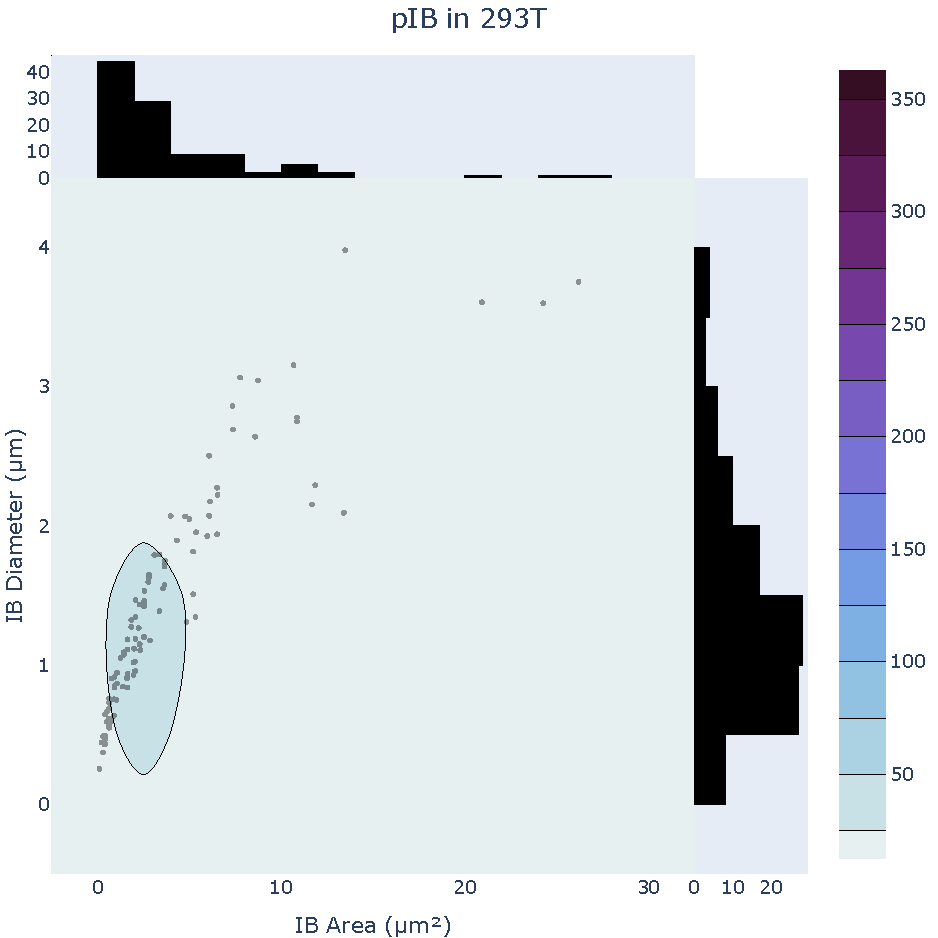
\includegraphics[width=\textwidth]{09. Chapter 4/Figs/03. pIB/00. pIB characterisation/01. heatmap_pib-293t.pdf} 
    \end{subfigure}
    \hfill
    \begin{subfigure}{0.495\textwidth}
        \caption{}
        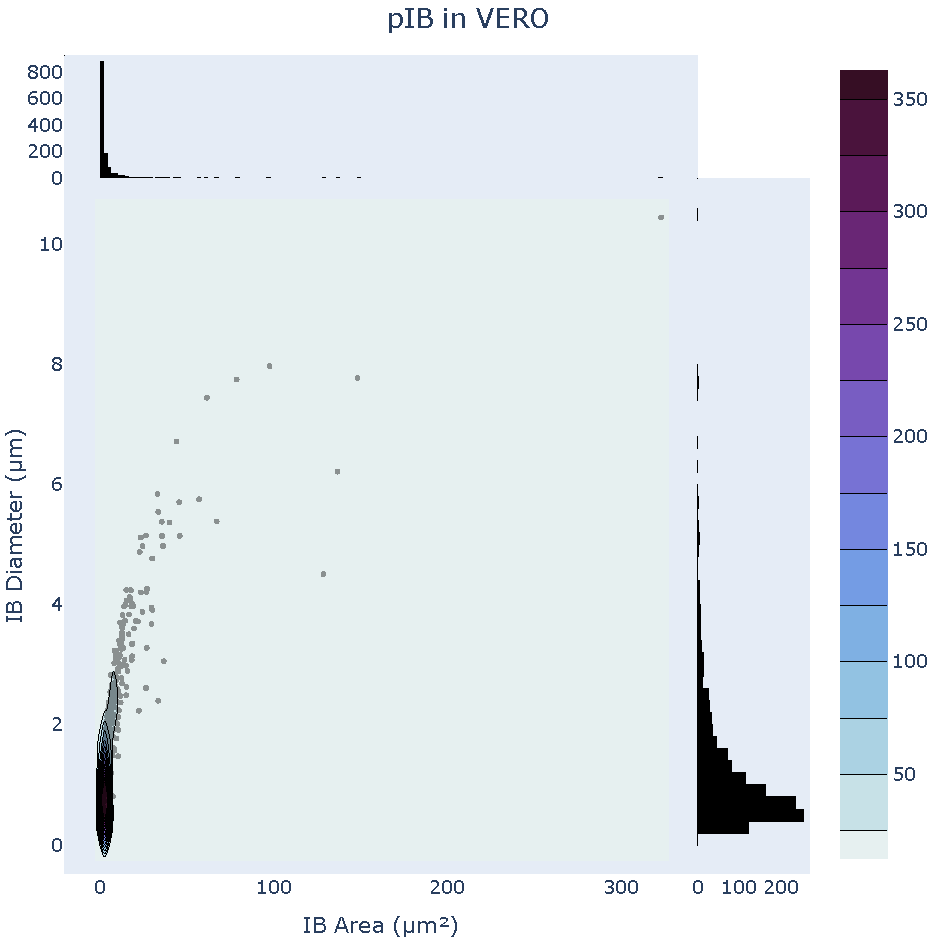
\includegraphics[width=\textwidth]{09. Chapter 4/Figs/03. pIB/00. pIB characterisation/02. heatmap_pib-vero.pdf}
    \end{subfigure}
    \caption[Size Characterization of Pseudo Inclusion Bodies Across Different Cell Lines.]{\textbf{Size Characterization of Pseudo Inclusion Bodies Across Different Cell Lines.} This figure presents the relationship between the measured area (\(\mu m^2\)) and diameter (\(\mu m\)) of individual pseudo inclusion bodies (pIBs) as observed within the scope of this study. Additionally, the figure includes distinct population distributions depicted alongside the plots, representing (a) 103
     o observations from the 293T cell line and (b) 1321 observations from the Vero cell line. Contour plots are incorporated to elucidate the underlying density of individual IBs within the plots.}
    \label{fig:Size Characterization of Pseudo Inclusion Bodies Across Different Cell Lines}
\end{figure}


\begin{figure}
    \centering
    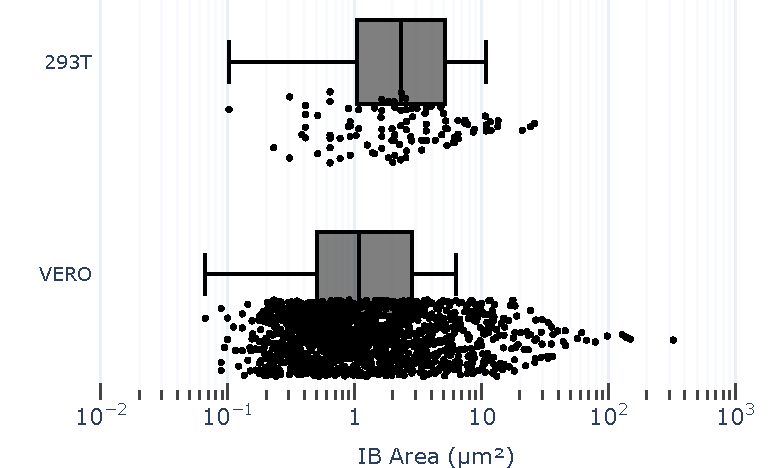
\includegraphics[width=1\linewidth]{09. Chapter 4/Figs/03. pIB/00. pIB characterisation/03. box-pib.pdf}
    \caption[boxplot of pib sizes per cell line.]{\textbf{boxplot of pib sizes per cell line.} this is the data from above but only area, to be able to compare it later}
    \label{fig:boxplot of pib sizes per cell line}
\end{figure}

\subsubsection{pIB IFIT1}

\begin{figure}
    \begin{subfigure}{0.495\textwidth}
        \caption{}
        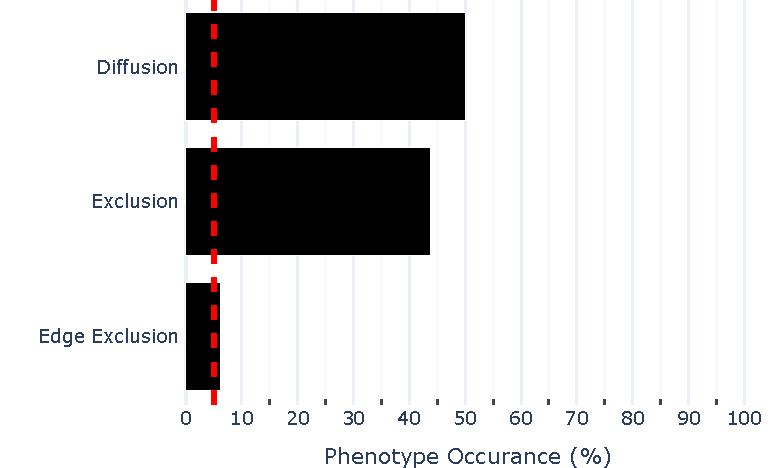
\includegraphics[width=1\linewidth]{09. Chapter 4/Figs/03. pIB/01. IFIT1/01. bar_i1_293t.pdf} 
    \end{subfigure}
    \begin{subfigure}{0.495\textwidth}
        \caption{}
        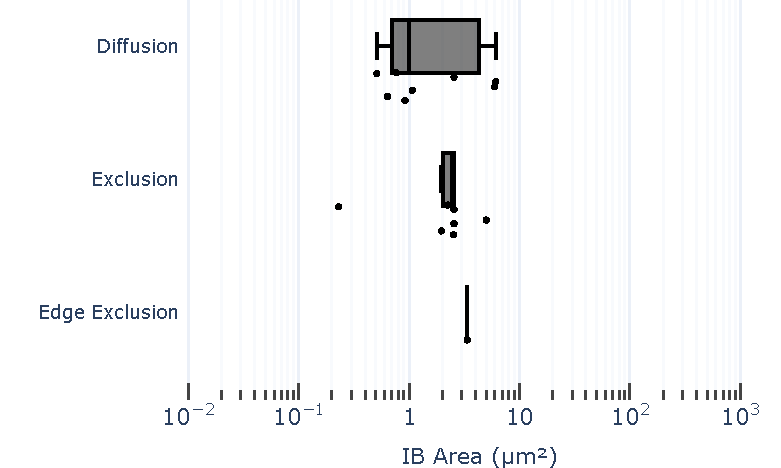
\includegraphics[width=1\linewidth]{09. Chapter 4/Figs/03. pIB/01. IFIT1/02. box_i1_293t.pdf}
    \end{subfigure}
    \caption[Diverse Phenotypic Interactions of Human IFIT1 with Human Pseudo Inclusion Bodies (pIBs) in the 293T Cell Line.]{\textbf{Diverse Phenotypic Interactions of Human IFIT1 with Human Pseudo Inclusion Bodies (pIBs) in the 293T Cell Line.} 293T cells were transfected with hRSV N and P containing plasmids using TransIT-X2 and were fixed after 24 hours. Cells were labeled with anti-RSV N and anti-IFIT1 antibodies and imaged on confocal microscope. Panel (a) shows percentual proportions of observed phenotypes between hRSV pseudo inclusion bodies and human IFIT1 (16 observations), with the red dotted line denoting the 5\% threshold, marking phenotypes considered relevant above this limit. Panel (b) shows the IB area in \(\mu m^2\) per observed relevant phenotype.}
    \label{fig:Diverse Phenotypic Interactions of Human IFIT1 with Human Pseudo Inclusion Bodies (pIBs) in the 293T Cell Line}
\end{figure}

\begin{figure}
    \centering
    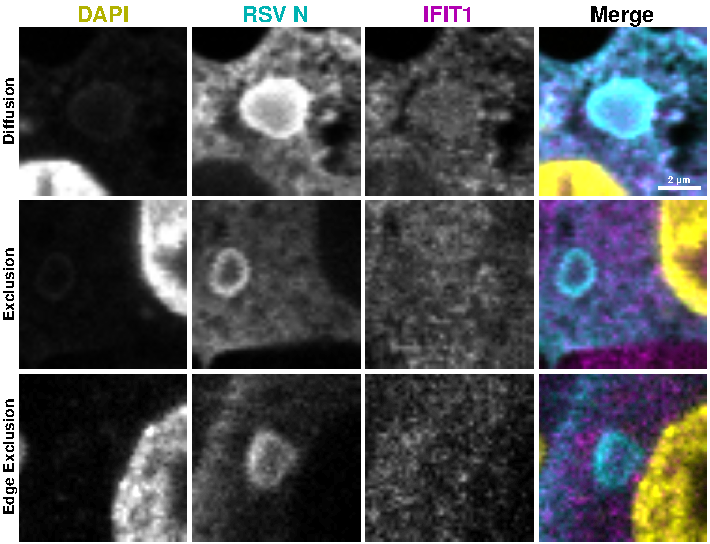
\includegraphics[width=1\linewidth]{09. Chapter 4/Figs/03. pIB/01. IFIT1/03. i1-293t-hnhp.pdf}
    \caption[Representative Images of Diverse Phenotypic Interactions of Human IFIT1 with Human Pseudo Inclusion Bodies (pIBs) in the 293T Cell Line.]{\textbf{Representative Images of Diverse Phenotypic Interactions of Human IFIT1 with Human Pseudo Inclusion Bodies (pIBs) in the 293T Cell Line.} 293T cells were transfected with hRSV N and P containing plasmids using TransIT-X2 and were fixed after 24 hours. Cellular nuclei were stained with DAPI (yellow), and cells were double-labeled with anti-RSV N (cyan) and anti-IFIT1 (magenta) antibodies. This figure showcases representative examples of relevant phenotypes in the interaction between human IFIT1 and hRSV pseudo inclusion bodies. These phenotypes are presented in descending order based on their percentage proportions. The scale bar indicates 2 \(\mu m\).}
    \label{fig:Representative Images of Diverse Phenotypic Interactions of Human IFIT1 with Human Pseudo Inclusion Bodies (pIBs) in the 293T Cell Line}
\end{figure}


Nascent human IFIT1 seems to be diffused through the pIB structure i.e., the signal intensity and distribution between cytoplasmic and pIB staining is identical.  

Endogenous monkey IFIT1 displays colocalization with human pIB structures (top panel), or inclusion within the structures (bottom panel). Monkey IFIT1 signal is also excluded from the pIB filamentous network (top panel; shown by arrows). This suggests that the colocalization is not caused by mere interaction with N or P but its dependant on the integrity of pIBs. These data are supported by z stack measurements.  

\begin{figure}
    \begin{subfigure}{0.495\textwidth}
        \caption{}
        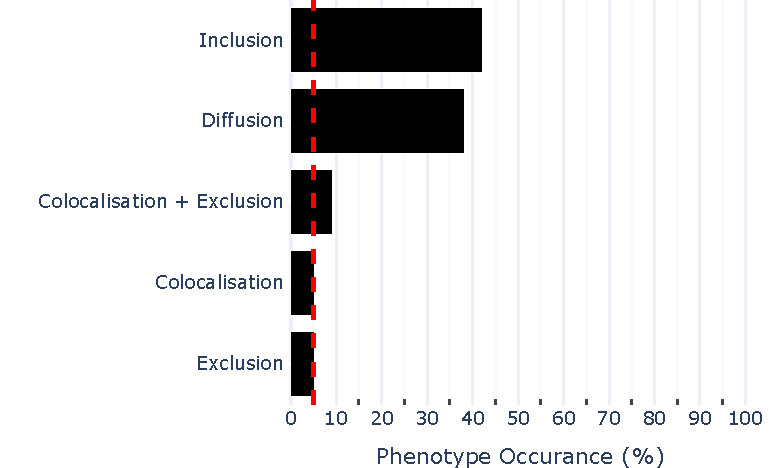
\includegraphics[width=1\linewidth]{09. Chapter 4/Figs/03. pIB/01. IFIT1/04. bar_i1_vero_hnhp.pdf} 
    \end{subfigure}
    \begin{subfigure}{0.495\textwidth}
        \caption{}
        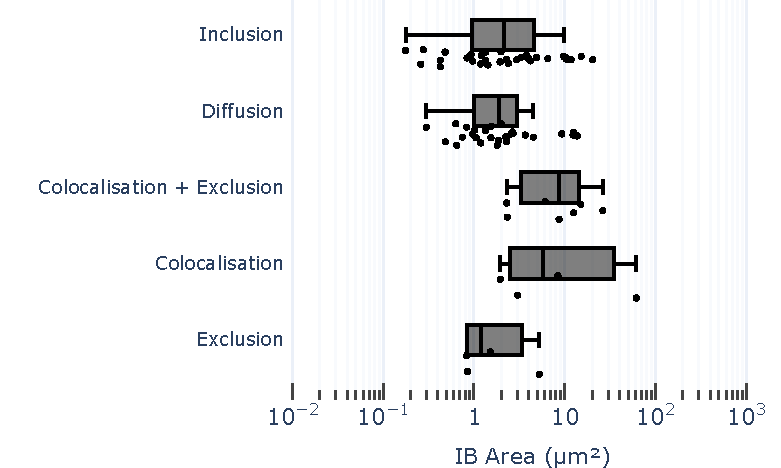
\includegraphics[width=1\linewidth]{09. Chapter 4/Figs/03. pIB/01. IFIT1/05. box_i1_vero_hnhp.pdf}
    \end{subfigure}
    \caption[Diverse Phenotypic Interactions of Monkey IFIT1 with Human Pseudo Inclusion Bodies (pIBs) in the VERO Cell Line.]{\textbf{Diverse Phenotypic Interactions of Monkey IFIT1 with Human Pseudo Inclusion Bodies (pIBs) in the VERO Cell Line.} Vero cells were transfected with hRSV N and P containing plasmids using TransIT-X2 and were fixed after 24 hours. Cells were labeled with anti-RSV N and anti-IFIT1 antibodies and imaged on confocal microscope. Panel (a) shows percentual proportions of observed phenotypes between hRSV pseudo inclusion bodies and monkey IFIT1 (76 observations), with the red dotted line denoting the 5\% threshold, marking phenotypes considered relevant above this limit. Panel (b) shows the IB area in \(\mu m^2\) per observed relevant phenotype.}
    \label{fig:Diverse Phenotypic Interactions of Monkey IFIT1 with Human Pseudo Inclusion Bodies (pIBs) in the VERO Cell Line}
\end{figure}

\begin{figure}
    \centering
    \includegraphics[width=1\linewidth]{09. Chapter 4/Figs/03. pIB/01. IFIT1/06. i1-vero-hnhp.pdf}
    \caption[Representative Images of Diverse Phenotypic Interactions of Monkey IFIT1 with Human Pseudo Inclusion Bodies (pIBs) in the VERO Cell Line.]{\textbf{Representative Images of Diverse Phenotypic Interactions of Monkey IFIT1 with Human Pseudo Inclusion Bodies (pIBs) in the VERO Cell Line.} Vero cells were transfected with hRSV N and P containing plasmids using TransIT-X2 and were fixed after 24 hours. Cellular nuclei were stained with DAPI (yellow), and cells were double-labeled with anti-RSV N (cyan) and anti-IFIT1 (magenta) antibodies. This figure showcases representative examples of relevant phenotypes in the interaction between monkey IFIT1 and hRSV pseudo inclusion bodies. These phenotypes are presented in descending order based on their percentage proportions. The scale bar indicates 2 \(\mu m\).}
    \label{fig:Representative Images of Diverse Phenotypic Interactions of Monkey IFIT1 with Human Pseudo Inclusion Bodies (pIBs) in the VERO Cell Line}
\end{figure}

In the context of bovine pIB structures, nascent monkey IFIT1 seems to colocalise with the edges of the structures (highlighted by the arrows). Consistent to human pIB data, nascent monkey IFIT1 is excluded from filamentous pIB network.

\begin{figure}
    \begin{subfigure}{0.495\textwidth}
        \caption{}
        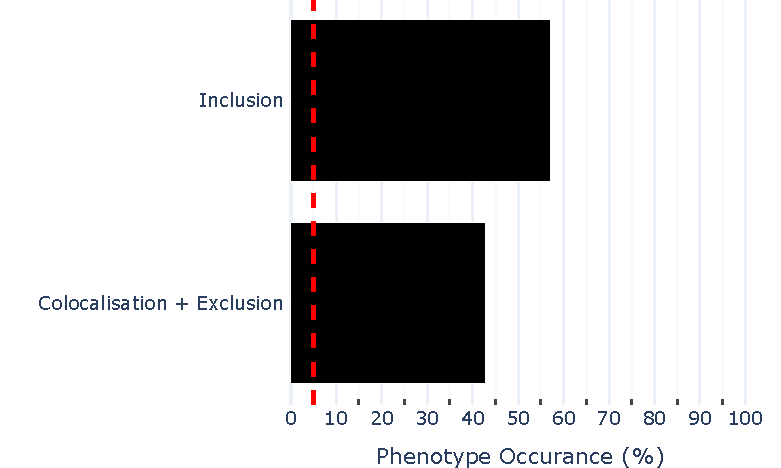
\includegraphics[width=1\linewidth]{09. Chapter 4/Figs/03. pIB/01. IFIT1/07. bar_i1_vero_bnbp.pdf}  
    \end{subfigure}
    \begin{subfigure}{0.495\textwidth}
        \caption{}
        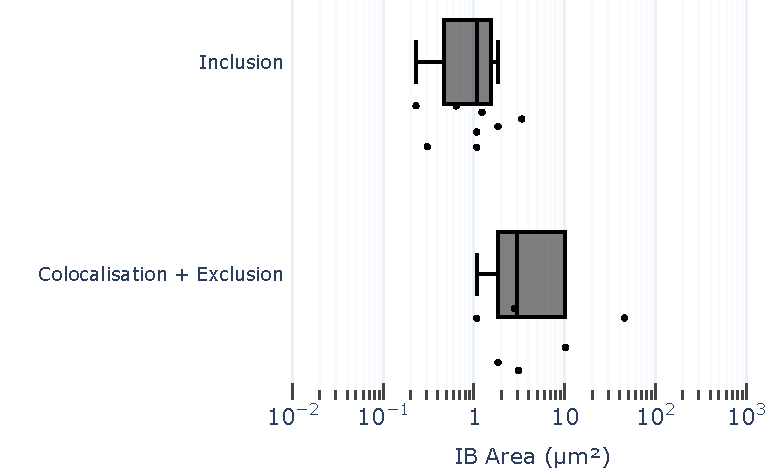
\includegraphics[width=1\linewidth]{09. Chapter 4/Figs/03. pIB/01. IFIT1/08. box_i1_vero_bnbp.pdf}
    \end{subfigure}
    \caption[Diverse Phenotypic Interactions of Monkey IFIT1 with Bovine Pseudo Inclusion Bodies (pIBs) in the VERO Cell Line.]{\textbf{Diverse Phenotypic Interactions of Monkey IFIT1 with Bovine Pseudo Inclusion Bodies (pIBs) in the VERO Cell Line.} Vero cells were transfected with bRSV N and P containing plasmids using TransIT-X2 and were fixed after 24 hours. Cells were labeled with anti-RSV N and anti-IFIT1 antibodies and imaged on confocal microscope. Panel (a) shows percentual proportions of observed phenotypes between bRSV pseudo inclusion bodies and monkey IFIT1 (14 observations), with the red dotted line denoting the 5\% threshold, marking phenotypes considered relevant above this limit. Panel (b) shows the IB area in \(\mu m^2\) per observed relevant phenotype.}
    \label{fig:Diverse Phenotypic Interactions of Monkey IFIT1 with Bovine Pseudo Inclusion Bodies (pIBs) in the VERO Cell Line}
\end{figure}

\begin{figure}
    \centering
    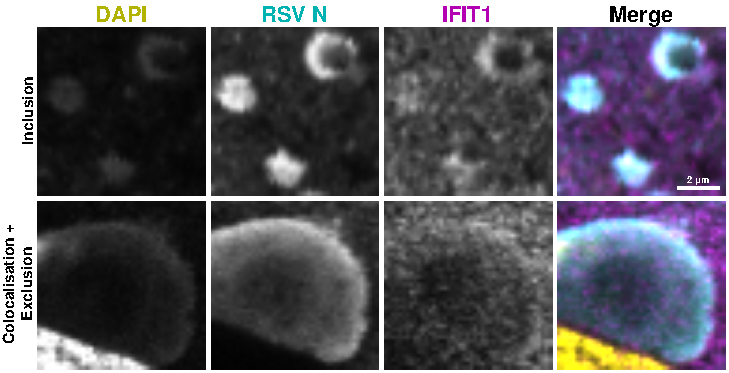
\includegraphics[width=1\linewidth]{09. Chapter 4/Figs/03. pIB/01. IFIT1/09. i1-vero-bnbp.pdf}
    \caption[Representative Images of Diverse Phenotypic Interactions of Monkey IFIT1 with Bovine Pseudo Inclusion Bodies (pIBs) in the VERO Cell Line.]{\textbf{Representative Images of Diverse Phenotypic Interactions of Monkey IFIT1 with Bovine Pseudo Inclusion Bodies (pIBs) in the VERO Cell Line.} Vero cells were transfected with bRSV N and P containing plasmids using TransIT-X2 and were fixed after 24 hours. Cellular nuclei were stained with DAPI (yellow), and cells were double-labeled with anti-RSV N (cyan) and anti-IFIT1 (magenta) antibodies. This figure showcases representative examples of relevant phenotypes in the interaction between monkey IFIT1 and bRSV pseudo inclusion bodies. These phenotypes are presented in descending order based on their percentage proportions. The scale bar indicates 2 \(\mu m\).}
    \label{fig:Representative Images of Diverse Phenotypic Interactions of Monkey IFIT1 with Bovine Pseudo Inclusion Bodies (pIBs) in the VERO Cell Line}
\end{figure}

\subsubsection{pIB IFIT3}
Nascent monkey IFIT3 seems to behave a if he pIB was not here. This means I has diffused phenotype. One exception is the top panel (shown with the arrow) which hints at concentrated IFIT3 at the edge of the pIBs. We do not know the localisation with respect to the pIB filaments as none were found in the slides. This data is as well supported by z stack measurements.

\begin{figure}
    \begin{subfigure}{0.495\textwidth}
        \caption{}
        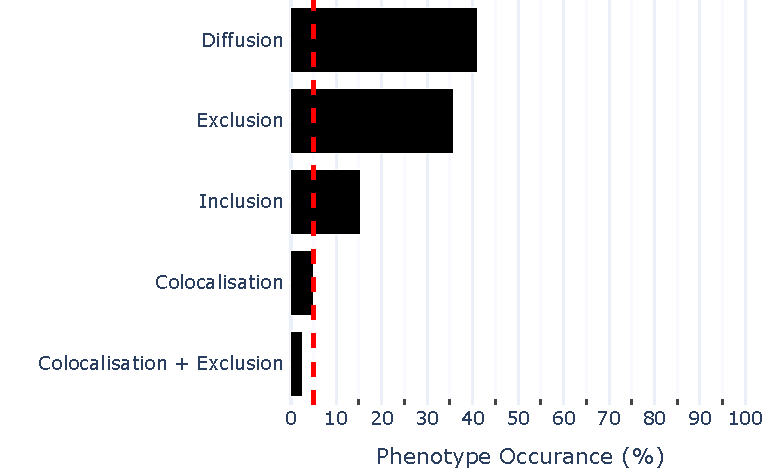
\includegraphics[width=1\linewidth]{09. Chapter 4/Figs/03. pIB/02. IFIT3/01. bar_i3_vero.pdf} 
    \end{subfigure}
    \begin{subfigure}{0.495\textwidth}
        \caption{}
        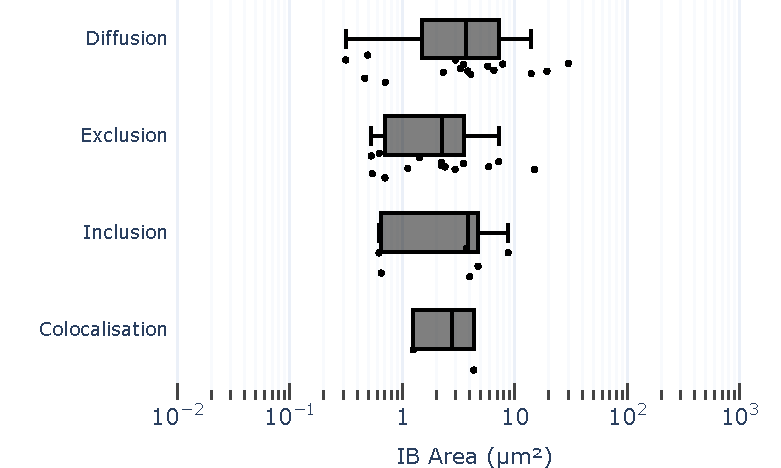
\includegraphics[width=1\linewidth]{09. Chapter 4/Figs/03. pIB/02. IFIT3/02. box_i3_vero.pdf}
    \end{subfigure}
    \caption[Diverse Phenotypic Interactions of Monkey IFIT3 with Human Pseudo Inclusion Bodies (pIBs) in the VERO Cell Line.]{\textbf{Diverse Phenotypic Interactions of Monkey IFIT3 with Human Pseudo Inclusion Bodies (pIBs) in the VERO Cell Line.} Vero cells were transfected with hRSV N and P containing plasmids using TransIT-X2 and were fixed after 24 hours. Cells were labeled with anti-RSV N and anti-IFIT3 antibodies and imaged on confocal microscope. Panel (a) shows percentual proportions of observed phenotypes between hRSV pseudo inclusion bodies and monkey IFIT3 (39 observations), with the red dotted line denoting the 5\% threshold, marking phenotypes considered relevant above this limit. Panel (b) shows the IB area in \(\mu m^2\) per observed relevant phenotype.}
    \label{fig:Diverse Phenotypic Interactions of Monkey IFIT3 with Human Pseudo Inclusion Bodies (pIBs) in the VERO Cell Line}
\end{figure}

\begin{figure}
    \centering
    \includegraphics[width=1\linewidth]{09. Chapter 4/Figs/03. pIB/02. IFIT3/03. i3-vero-hnhp.pdf}
    \caption[Representative Images of Diverse Phenotypic Interactions of Monkey IFIT3 with Human Pseudo Inclusion Bodies (pIBs) in the VERO Cell Line.]{\textbf{Representative Images of Diverse Phenotypic Interactions of Monkey IFIT3 with Human Pseudo Inclusion Bodies (pIBs) in the VERO Cell Line.} Vero cells were transfected with hRSV N and P containing plasmids using TransIT-X2 and were fixed after 24 hours. Cellular nuclei were stained with DAPI (yellow), and cells were double-labeled with anti-RSV N (cyan) and anti-IFIT3 (magenta) antibodies. This figure showcases representative examples of relevant phenotypes in the interaction between monkey IFIT3 and hRSV pseudo inclusion bodies. These phenotypes are presented in descending order based on their percentage proportions. The scale bar indicates 2 \(\mu m\).}
    \label{fig:Representative Images of Diverse Phenotypic Interactions of Monkey IFIT3 with Human Pseudo Inclusion Bodies (pIBs) in the VERO Cell Line}
\end{figure}

\subsubsection{pIB IFIT5}
Nascent monkey IFIT5 colocalises with hRSV pseudo inclusion bodies (basically resembling the P staining). It also colocalises with pIB filamentous network. This network is only seen in cells that are co-transfected with RSV N and P proteins. We believe that they are an aftermath of a pIB breakdown. This data is as well supported by z stack measurements.

\begin{figure}
    \begin{subfigure}{0.495\textwidth}
        \caption{}
        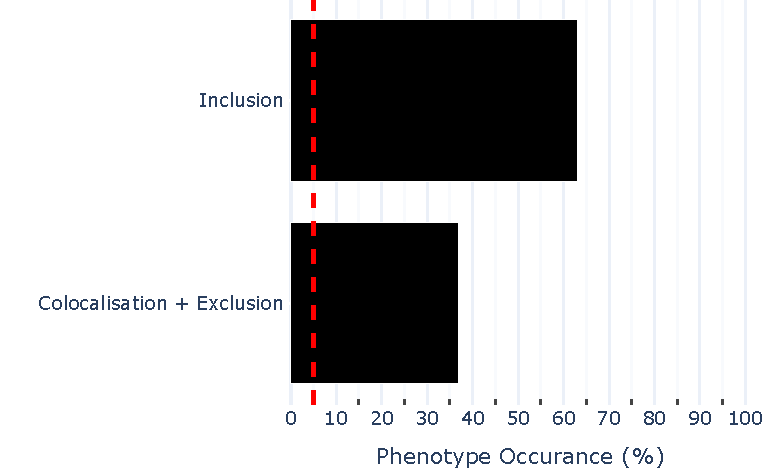
\includegraphics[width=1\linewidth]{09. Chapter 4/Figs/03. pIB/03. IFIT5/01. bar_i5_vero.pdf} 
    \end{subfigure}
    \begin{subfigure}{0.495\textwidth}
        \caption{}
        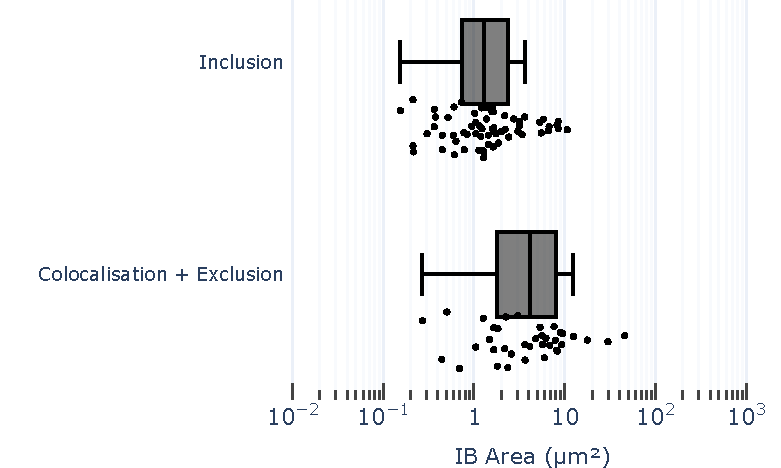
\includegraphics[width=1\linewidth]{09. Chapter 4/Figs/03. pIB/03. IFIT5/02. box_i5_vero.pdf}
    \end{subfigure}
    \caption[Diverse Phenotypic Interactions of Monkey IFIT5 with Human Pseudo Inclusion Bodies (pIBs) in the VERO Cell Line.]{\textbf{Diverse Phenotypic Interactions of Monkey IFIT5 with Human Pseudo Inclusion Bodies (pIBs) in the VERO Cell Line.} Vero cells were transfected with hRSV N and P containing plasmids using TransIT-X2 and were fixed after 24 hours. Cells were labeled with anti-RSV N and anti-IFIT5 antibodies and imaged on confocal microscope. Panel (a) shows percentual proportions of observed phenotypes between hRSV pseudo inclusion bodies and monkey IFIT5 (100 observations), with the red dotted line denoting the 5\% threshold, marking phenotypes considered relevant above this limit. Panel (b) shows the IB area in \(\mu m^2\) per observed relevant phenotype.}
    \label{fig:Diverse Phenotypic Interactions of Monkey IFIT5 with Human Pseudo Inclusion Bodies (pIBs) in the VERO Cell Line}
\end{figure}

\begin{figure}
    \centering
    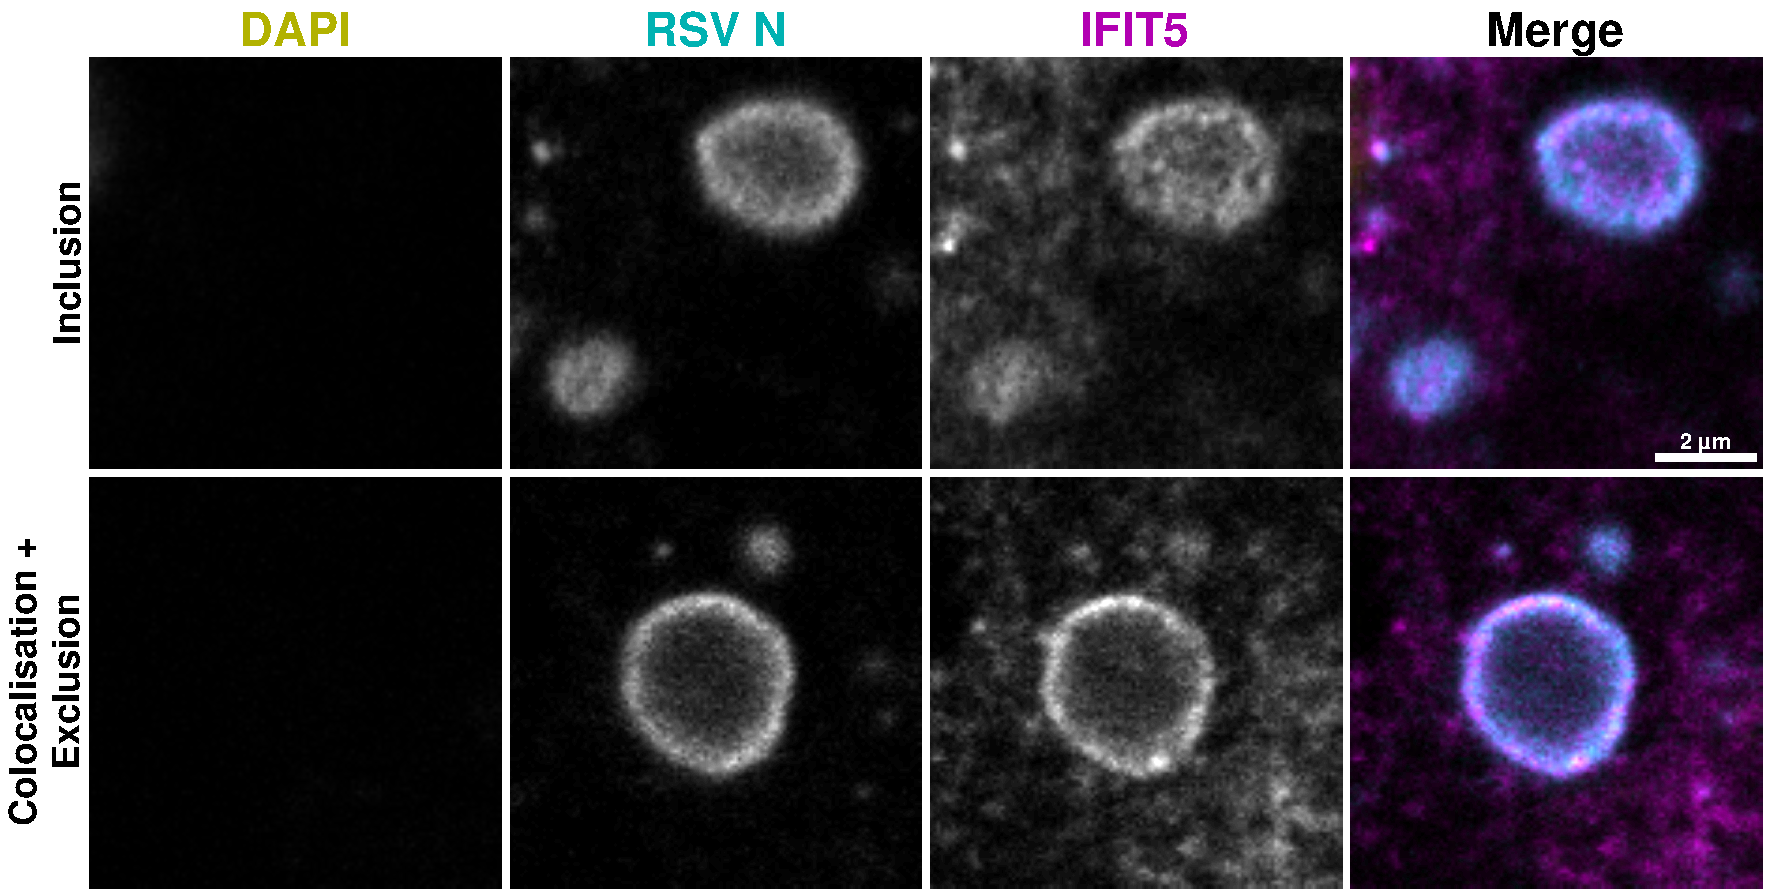
\includegraphics[width=1\linewidth]{09. Chapter 4/Figs/03. pIB/03. IFIT5/03. i5-vero-hnhp.pdf}
    \caption[Representative Images of Diverse Phenotypic Interactions of Monkey IFIT5 with Human Pseudo Inclusion Bodies (pIBs) in the VERO Cell Line.]{\textbf{Representative Images of Diverse Phenotypic Interactions of Monkey IFIT5 with Human Pseudo Inclusion Bodies (pIBs) in the VERO Cell Line.} Vero cells were transfected with hRSV N and P containing plasmids using TransIT-X2 and were fixed after 24 hours. Cellular nuclei were stained with DAPI (yellow), and cells were double-labeled with anti-RSV N (cyan) and anti-IFIT5 (magenta) antibodies. This figure showcases representative examples of relevant phenotypes in the interaction between monkey IFIT5 and hRSV pseudo inclusion bodies. These phenotypes are presented in descending order based on their percentage proportions. The scale bar indicates 2 \(\mu m\).}
    \label{fig:Representative Images of Diverse Phenotypic Interactions of Monkey IFIT5 with Human Pseudo Inclusion Bodies (pIBs) in the VERO Cell Line}
\end{figure}

\subsubsection{Summary} \label{Summary-pib}
Endogenous human IFIT1 seems to be diffused through the human pIB structure. On the other hand, endogenous monkey IFIT1 forms an inclusion in human pIBs, colocalises with the edge of human and bovine pIBs and is excluded from the filamentous pIB network. This suggests that the colocalization is not caused by mere interaction with N or P but its dependant on the integrity of pIBs.

Endogenous monkey IFIT3 seems to be diffuse through the human pIB structures (with maybe a small hint of colocalization).

Endogenous monkey IFIT5 colocalises with human pIBs and with the NP network (this network is never present in infected cells, so we do not know how are other IFIT5s colocalising with it).